%=====================================================================
\section{結果}
\label{sec:results}
表\ref{tab:measured} に単一ストリームの代表値と，同時実行スイープでの最大スループットをまとめる．

\begin{table}[htbp]\centering\small
\caption{実測サマリ．TTFT は約 1k と 32k トークンのプロンプト（ms）．prefill MFU（Model FLOPs Utilization）は 8k トークン超のプロンプトでの（モデル FLOPs / TTFT）/ 835\,TFLOPS．
TPOT は 2k トークン未満のプロンプトの中央値（ms），TPOT$_{min}$ は同条件の理論下限，HBM util. は（理論読み出しバイト / TPOT）/ 3.9\,TB/s．
MTP 列は $\gamma=4$ の TPOT 高速化（中央値）とmean acceptance length AL（Synthetic + SWE-bench）．max out tok/s は同時実行スイープでの最大出力スループット．}
\label{tab:measured}
\begin{adjustbox}{max width=\linewidth}
\begin{tabular}{lrrrrrrrrr}
\toprule
Model & TTFT 1k & TTFT 32k & prefill MFU & TPOT & TPOT$_{min}$ & HBM util. & MTP speedup & AL & max out tok/s \\
\midrule
Gemma4 E2B & 22 & 602 & 36\% & 4.21 & 1.19 & 28\% & 1.94$\times$ & 2.78 & 6869 \\
Gemma4 E4B & 25 & 896 & 43\% & 6.23 & 2.42 & 39\% & 2.17$\times$ & 2.90 & 4264 \\
Gemma4 12B & 42 & 2203 & 47\% & 10.41 & 6.19 & 59\% & 1.85$\times$ & 3.20 & 1659 \\
Gemma4 26B-A4B & 35 & 1051 & 33\% & 5.30 & 2.00 & 38\% & 1.35$\times$ & 3.46 & 2392 \\
Gemma4 31B & 104 & 5999 & 45\% & 22.87 & 15.91 & 70\% & 3.08$\times$ & 3.58 & 533 \\
Qwen3-30B-A3B & 45 & 1563 & 41\% & 4.56 & 1.58 & 35\% & -- & -- & 2599 \\
Qwen3-32B & 106 & 7179 & 49\% & 22.01 & 16.45 & 75\% & -- & -- & 839 \\
\bottomrule
\end{tabular}

\end{adjustbox}
\end{table}

%---------------------------------------------------------------------
\subsection{Prefill：Hybrid Attentionは長いプロンプトで効く}
\label{sec:prefill}
\paragraph{大きい dense モデルは本機の GEMM 性能をほぼ使い切っている．}
2k トークン以上の実効 FLOP レートは 12B/31B/Qwen3-32B で 380--415\,TFLOPS にそろう（図\ref{fig:prefill-rate}）．
データシート値の 45--49\% だが，本機の実測 GEMM ピーク（492--514\,TFLOPS，表\ref{tab:hw}）に対しては 74--84\% に当たる．
一方 MoE は 8k トークン超でも 26B-A4B が 265--277\,TFLOPS，Qwen3-30B-A3B が 305--356\,TFLOPS にとどまる．
expert ごとの GEMM（中間次元 704 など）は小さく，プロンプトのトークンが 128 個の expert に分散するため，1 つの GEMM あたりの行数も少なくなるからである．

\begin{figure}[htbp]\centering
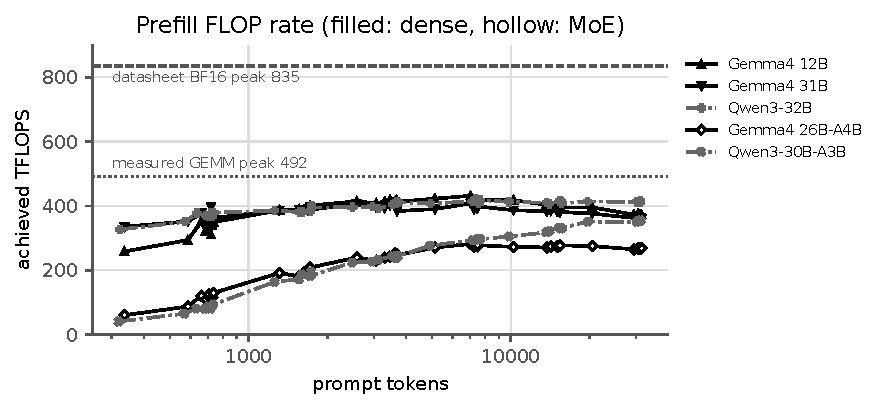
\includegraphics[width=0.6\linewidth]{prefill_rate.pdf}
\caption{prefill の実効 FLOP レート（モデル FLOPs / TTFT）．塗りは dense，白抜きは MoE．破線はデータシート値，点線は本機の実測 GEMM ピーク（初回の計測値 492\,TFLOPS）．}
\label{fig:prefill-rate}
\end{figure}

\paragraph{Hybrid Attentionは長いプロンプトで効く．}
sliding window の効果を確かめるため，同クラスの Qwen3 に対する TTFT の比を，式\eqref{eq:prefill}の FLOPs の比と並べた（図\ref{fig:prefill-hybrid}）．
点線は Gemma~4 の全層を global とした場合の FLOPs の比で，実線との差が sliding window で減った分である．
\begin{itemize}
\item \textbf{window size（1024）以下では差がない．}このとき local 層も全トークンを参照するので，Attentionの FLOPs は Gemma~4 と全層 global で同じになる．
      dense の組では TTFT の比は 0.95--0.98 で，パラメータ数の差による FLOPs の比（0.94）とほぼ一致する．
\item \textbf{効果が見えるのは 4k トークン以上である．}window sizeを超えても，Attentionが prefill の FLOPs に占める割合は 2k トークンで 3\% 程度と小さく，
      sliding window で削れる量も小さい．$P^2$ で増えるAttentionの割合が大きくなる 4k 以上で，実線と点線が離れ，測った TTFT の比も下がっていく．
\item \textbf{32k では 31B が 16\%，26B-A4B が 33\% 速い．}TTFT は 31B が 6.0\,s 対 7.2\,s，26B-A4B が 1.05\,s 対 1.56\,s である．
      Attentionが FLOPs に占める割合は，Qwen3-32B の 36\% に対し 31B は 18\% である．
\end{itemize}
ただし 32k での実測の比（0.84，0.68）は FLOPs の比（0.73，0.51）ほど下がらない．
31B の実効 FLOP レートは 32k で Qwen3-32B より 1 割ほど低く（図\ref{fig:prefill-rate}），Gemma~4 のAttention計算（head dim 512 を含む FA4 系カーネル）の効率が Qwen3 の FlashAttention 3 より低い可能性がある．
また 26B-A4B はwindow size以下の短いプロンプトで FLOPs が多いのに Qwen3-30B-A3B より 15--20\% 速い．この領域の TTFT は 35--50\,ms で計算量では決まっておらず，Attentionとは別の要因である．

\begin{figure}[htbp]\centering
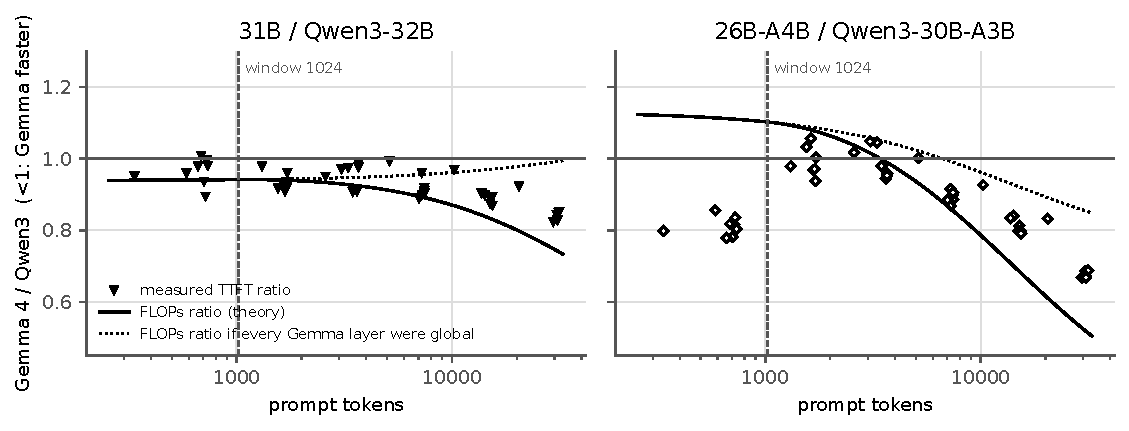
\includegraphics[width=\linewidth]{prefill_hybrid.pdf}
\caption{同クラスの Qwen3 に対する TTFT の比（点）と prefill FLOPs の比（実線）．点線は Gemma~4 の全層を global とした場合の FLOPs の比．破線はwindow size 1024．}
\label{fig:prefill-hybrid}
\end{figure}

%---------------------------------------------------------------------
\subsection{短いコンテキストの decode：大きいモデルほど理論値に近い}
\label{sec:short}
図\ref{fig:decode-bw} のとおり，1 ステップで読むバイト数が大きいモデルほど理論帯域に近い．

\begin{figure}[htbp]\centering
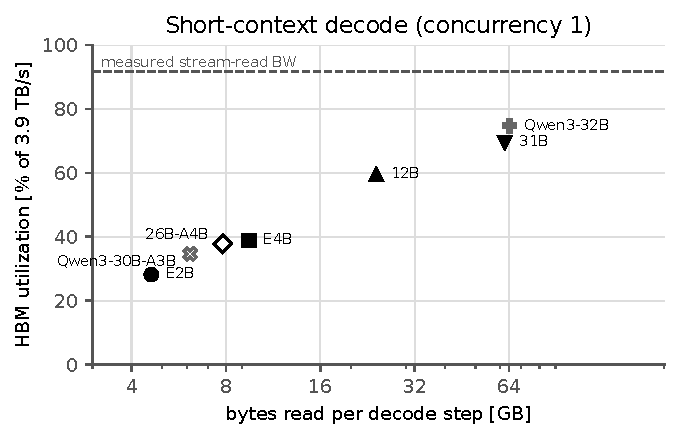
\includegraphics[width=0.6\linewidth]{decode_bw.pdf}
\caption{短いコンテキスト（2k トークン未満）の decode における，1 ステップの読み出しバイト（式\eqref{eq:bytes}）と HBM 利用率．}
\label{fig:decode-bw}
\end{figure}

理由を調べるため，Nsight Systems で測った decode 1 ステップの時間を，
「重みを実測帯域（3.57\,TB/s）で読む理想時間」と，それを超える部分に分けた（図\ref{fig:decode-gap}，表\ref{tab:nsys}）．
\textbf{理想時間を超える部分は，モデルの大きさによらず 1 ステップ 2.7--4.6\,ms ある．}
31B ではこれが理想時間 17.2\,ms の 27\% にすぎないが，E2B では理想時間 1.3\,ms の 2 倍になる．
小さいモデルの帯域利用率が低いのは，この一定の上乗せが相対的に重いためである．

\begin{figure}[htbp]\centering
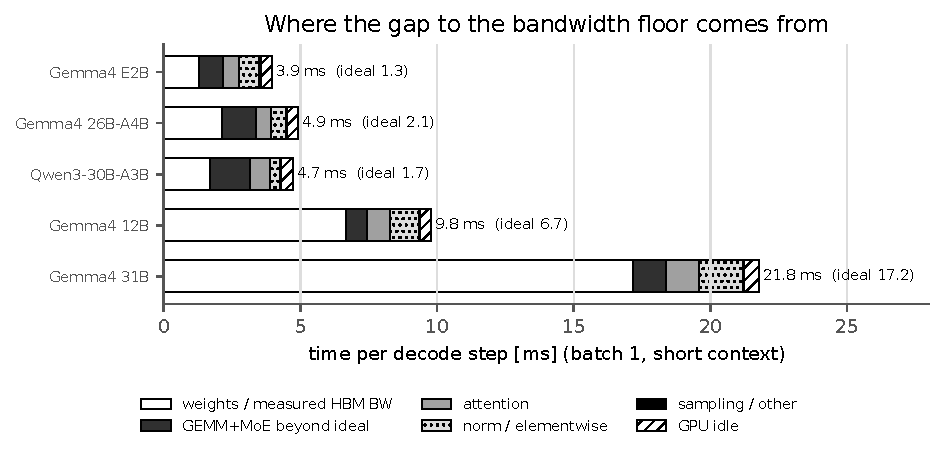
\includegraphics[width=0.85\linewidth]{decode_gap.pdf}
\caption{decode 1 ステップの時間の分解（Nsight Systems，バッチ 1，短いコンテキスト）．白は重みを実測 HBM 帯域で読む理想時間で，それ以外が帯域律速の下限からの差．}
\label{fig:decode-gap}
\end{figure}

上乗せの中身は次のとおりで，いずれも「1 個あたり数 µs かかるカーネルが 1 ステップに数百個並ぶ」ことに由来する．
CUDA Graph により CPU からのカーネル起動のコストはほぼ消えているが，GPU 上でカーネル 1 個ごとにかかる起動・終了の時間とカーネル間の隙間は残る．



\begin{table}[htbp]\centering\small
\caption{decode 1 ステップの時間内訳（ms，バッチ 1，短いコンテキスト）．実効帯域 = 理論重みバイト / GEMM+MoE 時間．}
\label{tab:nsys}
\begin{tabular}{lrrrrrr}\toprule
 & step & GEMM+MoE & 実効帯域 & attention & norm/elem. & idle \\\midrule
Gemma4 E2B & 3.98 & 2.15 & 2.14\,TB/s & 0.61 & 0.74 & 0.40 \\
Gemma4 12B & 9.79 & 7.43 & 3.21\,TB/s & 0.86 & 1.03 & 0.41 \\
Gemma4 26B-A4B & 4.91 & 3.38 & 2.26\,TB/s & 0.52 & 0.56 & 0.40 \\
Gemma4 31B & 21.78 & 18.39 & 3.34\,TB/s & 1.19 & 1.60 & 0.55 \\
Qwen3-30B-A3B & 4.72 & 3.17 & 1.92\,TB/s & 0.73 & 0.34 & 0.44 \\\bottomrule
\end{tabular}
\end{table}

\begin{figure}[htbp]\centering
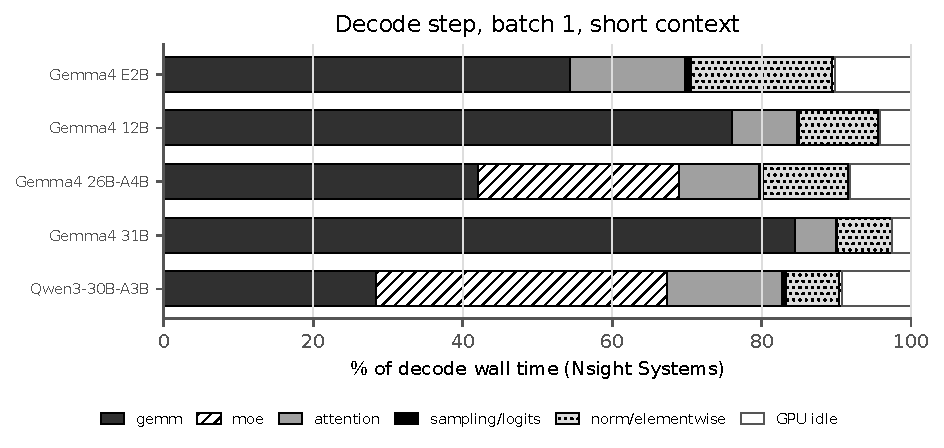
\includegraphics[width=0.85\linewidth]{nsys_short.pdf}
\caption{decode 1 ステップの時間内訳（Nsight Systems，バッチ 1，短いコンテキスト）．白は GPU idle．}
\label{fig:nsys-short}
\end{figure}

\begin{itemize}
\item \textbf{31B の GEMM は帯域をほぼ使い切っている．}重み 61\,GB を 18.4\,ms で読み，3.34\,TB/s（実測ピークの 94\%）に達する．
      TPOT 全体では理論帯域の 70\% で，残りはnormalizationなど（1.6\,ms），Attention（1.2\,ms），idle（0.55\,ms）である．
\item \textbf{E2B は GEMM 自体も帯域を使い切れない．}1 トークンあたり約 585 個のカーネルが走る．
      Nsight Systems によると，最も時間を使う GEMM カーネルは 1 回 6\,µs，grid は平均 43 CTA である．
      \S\ref{sec:gpu-model} で見たとおり，132 SM のうち 89 個に仕事がなく，1 wave で終わってしまう（図\ref{fig:smfill}(a)）．
      hidden 1536 の行列は小さく，CTA に分けても SM の数に届かないためで，GEMM は理想時間より 0.86\,ms 長い．
      さらに RMSNorm やresidual addなどの小さなカーネルが 0.74\,ms，35 層分のAttentionが 0.60\,ms，GPU idleが 0.40\,ms かかる．
\item \textbf{MoE の expert 計算は帯域効率が低い．}26B-A4B と Qwen3-30B-A3B では GEMM+MoE が理想時間より 1.2--1.5\,ms 長く，実効帯域は 1.9--2.3\,TB/s にとどまる．expert 1 つあたりの行列（$704 \times 2816$ など）が小さいためである．
\end{itemize}

\paragraph{GEMM 1 個ごとの固定時間（E9）．}
この上乗せをハードウェアの側から確かめるため，decode と同じ $M=1$ の GEMM を CUDA Graph の中で重みの大きさを変えて測った（図\ref{fig:gemv}）．
重みは L2（60\,MiB）より大きな組を巡回させ，毎回 HBM から読ませている．
時間は $t \approx 3.8\,\mu\text{s} + W / 3.46\,\text{TB/s}$（$W$ は重みのバイト数，$K=1536$ で最小二乗）でよく近似できる．
空のカーネルは 1.1\,µs なので，残りの約 2.7\,µs は最初のデータが HBM から届くまでの latency と，CTA が少なく帯域が立ち上がりきらない時間である．
このため 6\,MB の行列では 1.1\,TB/s しか出ず，HBM 帯域に近づくには 1 回で 50\,MB 以上を読む必要がある．
1 ステップの GEMM の数は E2B が 212 個，12B が 193 個，31B が 241 個で，モデルの大きさによらずほぼ同じである．
この式で 1 ステップの GEMM 時間を予測すると，E2B が 2.13\,ms（実測 2.15\,ms），12B が 7.6\,ms（7.4\,ms），31B が 18.7\,ms（18.4\,ms）で，3\% 以内で一致する．
固定分は E2B では 0.80\,ms で重みの読み出し（1.33\,ms）の 6 割に当たるが，31B では 0.91\,ms で 17.7\,ms の 5\% にすぎない．
\textbf{小さいモデルの帯域利用率が低いのは，約 200 個の GEMM がそれぞれ約 4\,µs の固定時間を払い，読むバイト数が少ないほどその比率が大きくなるからである．}

\begin{figure}[htbp]\centering
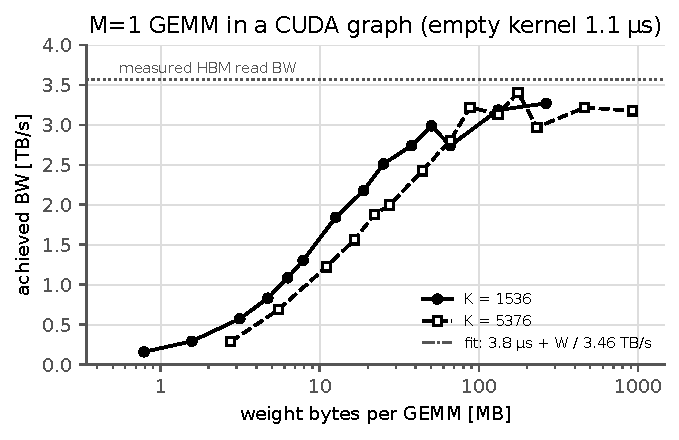
\includegraphics[width=0.6\linewidth]{gemv_bw.pdf}
\caption{$M=1$ の GEMM（CUDA Graph 内，重みは毎回 HBM から読む）の重みの大きさと達成帯域．一点鎖線は $K=1536$ での $t = t_0 + W/\text{BW}$ の当てはめ．}
\label{fig:gemv}
\end{figure}

%---------------------------------------------------------------------
\subsection{長いコンテキストの decode：Attentionカーネルの split-KV のバグ}
\label{sec:ctx}
コンテキスト長に対する TPOT の増え方は，Gemma と Qwen で大きく異なる（図\ref{fig:decode-long}，表\ref{tab:ctx}）．
Qwen3 の増分は KV 読み出しの理論増分の 1.3--1.4 倍に収まるが，Gemma~4 は 26--120 倍である．
理論下限（点線）はどちらもほぼ平らなので，この増分は KV の読み出し量では説明できない．
以下で示すとおり，原因は vLLM 0.32.0 の FlashAttention-4 カーネルの split-KV のバグで，1 行の修正で増分はほぼ理論値まで下がる（表\ref{tab:ctx} の右 2 列）．

\begin{figure}[htbp]\centering
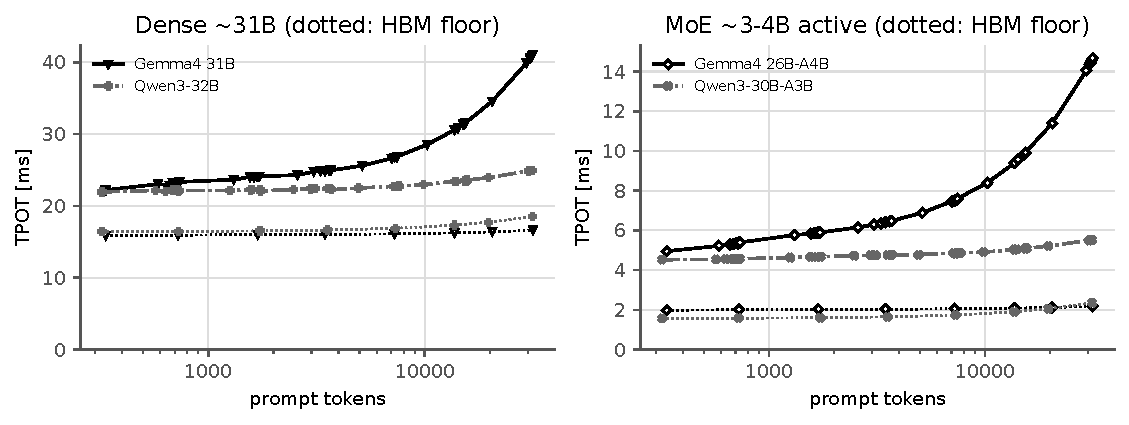
\includegraphics[width=\linewidth]{decode_long.pdf}
\caption{TPOT とプロンプト長．同クラスの Gemma~4 と Qwen3 の比較（点線は式\eqref{eq:bytes}による帯域律速の下限）．}
\label{fig:decode-long}
\end{figure}

\begin{table}[htbp]\centering\small
\caption{TPOT のコンテキスト長依存性（ms）．理論増分は KV 読み出しの増分 / 3.9\,TB/s．
右 2 列は split-KV を修正した FA4（\S\ref{sec:ctx-fix}）で同じ条件を測り直した値（E9）．}
\label{tab:ctx}
\begin{tabular}{lrrrrrr}\toprule
 & \multicolumn{3}{c}{vLLM 0.32.0} & & \multicolumn{2}{c}{split-KV 修正後} \\\cmidrule(lr){2-4}\cmidrule(lr){6-7}
モデル & TPOT（<1k） & TPOT（$\sim$30k） & 増分 & 理論増分 & TPOT（$\sim$30k） & 増分 \\\midrule
Gemma4 E2B & 4.21 & 16.96 & +12.8 & +0.11 & 3.70 & +0.11 \\
Gemma4 E4B & 6.23 & 19.02 & +12.8 & +0.22 & 5.79 & +0.26 \\
Gemma4 12B & 10.41 & 23.96 & +13.6 & +0.15 & 9.93 & +0.21 \\
Gemma4 26B-A4B & 5.30 & 14.44 & +9.1 & +0.17 & 4.87 & +0.14 \\
Gemma4 31B & 22.96 & 40.66 & +17.7 & +0.69 & 23.27 & +1.25 \\
Qwen3-30B-A3B & 4.56 & 5.52 & +1.0 & +0.77 & -- & -- \\
Qwen3-32B & 22.01 & 24.93 & +2.9 & +2.05 & -- & -- \\\bottomrule
\end{tabular}
\end{table}

\paragraph{どのカーネルが遅いか（Nsight Systems）．}
E2B の 30k トークン後の decode では，1 ステップ 19.0\,ms の 79\% をAttentionカーネルが占める（図\ref{fig:nsys-long}）．
同じ FlashAttention-4 カーネルが local 層では 1 回 23\,µs，global 層では 1 回 1.84\,ms かかる．
global 層 1 回で読む KV は約 61\,MB なので，実効帯域は約 33\,GB/s（HBM の 1\%）にすぎない．
31B（約 26k トークン）でも global 層は 1 回 1.56\,ms で，KV ヘッドが E2B の 4 倍あるのに時間はほぼ同じである．
\textbf{時間を決めているのは読むバイト数ではない}ことを示している．
vLLM は head dim が 256 と 512 の層が混在する Gemma~4 に対して全層で FlashAttention-4 を使っており，global 層の decode もこの経路を通る．
理由はコード\ref{lst:fa4}のとおりで，Hopper 既定の FlashAttention 3 は head dim 256 までしか扱えないため，BF16 の KV キャッシュでは FA4 を全層に使う．
FP8 の KV キャッシュを使う場合だけ，head dim 256 の local 層に FA3 を使う層ごとの選択に切り替わる（global 層は FA4 のまま．結果は後述）．

\lstinputlisting[float=htbp, caption={vLLM が Gemma~4 のAttentionカーネルを選ぶ処理（抜粋）．}, label={lst:fa4}]{code/fa4.py}


\begin{figure}[htbp]\centering
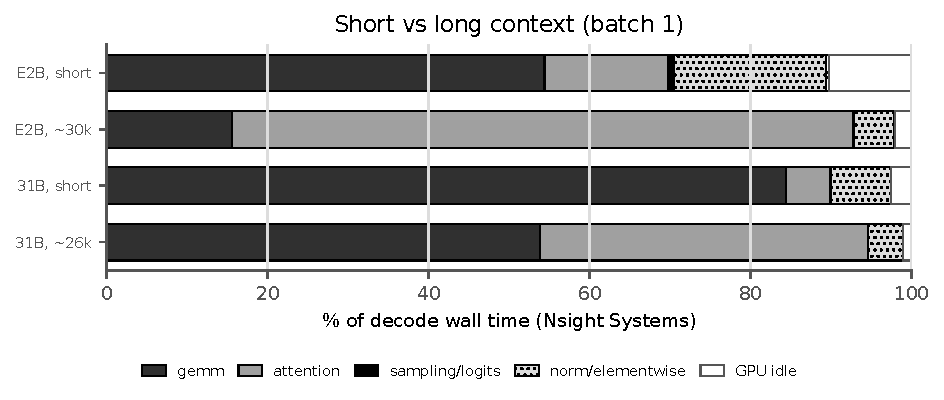
\includegraphics[width=0.85\linewidth]{nsys_long.pdf}
\caption{短いコンテキストと長いコンテキストでの decode 1 ステップの時間内訳（Nsight Systems，バッチ 1）．}
\label{fig:nsys-long}
\end{figure}

表\ref{tab:attn-bw} に，Attentionカーネル 1 回の時間を KV の読み出し量と比べた．
Gemma~4 の global 層は KV を理論帯域で読む時間の 28--117 倍かかり，実効帯域は 33--137\,GB/s にすぎない．
一方 Qwen3-32B（FlashAttention 3，head dim 128）は，26k トークンで 1 層あたり 106\,MB の KV を 44\,µs で読んでおり，実効帯域は 2.4\,TB/s である（split-KV の部分結果をまとめるカーネル 5\,µs を含めても 2.2\,TB/s）．
\textbf{読むバイト数が少ないのに遅いのは，モデルの設計ではなく，Gemma~4 の global 層に使われているAttentionカーネルの実装に原因がある．}

\begin{table}[htbp]\centering\small
\caption{長いコンテキストの decode におけるAttentionカーネル 1 回の時間と KV の読み出し量．理論時間は KV / 3.9\,TB/s．
Gemma~4 は CuTe DSL の FA（FA4 系），Qwen3-32B は FlashAttention 3．修正後の時間は split の部分結果をまとめる combine カーネルを含む（E9）．}
\label{tab:attn-bw}
\begin{tabular}{llrrrrrr}\toprule
 & & & & \multicolumn{2}{c}{vLLM 0.32.0} & \multicolumn{2}{c}{split-KV 修正後} \\\cmidrule(lr){5-6}\cmidrule(lr){7-8}
モデル & 層 & KV / 回 & 理論 & 実測 & 実効帯域 & 実測 & 実効帯域 \\\midrule
Gemma4 E2B（30k） & global & 61\,MB & 16\,µs & 1.84\,ms & 33\,GB/s & 44\,µs & 1.4\,TB/s \\
Gemma4 E2B（30k） & local & 0.5\,MB & 0.1\,µs & 23\,µs & 22\,GB/s & 15\,µs & 33\,GB/s \\
Gemma4 31B（26k） & global & 213\,MB & 55\,µs & 1.56\,ms & 137\,GB/s & 98\,µs & 2.2\,TB/s \\
Gemma4 31B（26k） & local & 17\,MB & 4\,µs & 38\,µs & 440\,GB/s & 23\,µs & 0.74\,TB/s \\
Qwen3-32B（26k） & 全層 & 106\,MB & 27\,µs & 44\,µs & 2.4\,TB/s & -- & -- \\\bottomrule
\end{tabular}
\end{table}

\paragraph{なぜ遅いか（Nsight Compute）．}
global 層のカーネルは理論どおりの 61.6\,MB を読んでおり，余計な読み出しはない（表\ref{tab:ncu}）．
しかし DRAM も SM もピークの 1\% 未満しか使っておらず，メモリ律速でも計算律速でもない．
grid は 128 CTA で SM の数に近いので，一見すると SM は埋まっているように見える．
ところが同じカーネルを単独で Nsight Compute にかけ，SM ごとの稼働サイクル（\texttt{sm\_\_cycles\_active}）を見ると，
最大の SM は 274 万サイクルとカーネルの実行時間（305 万サイクル）のほぼ全体で動いているのに，平均は 3.6 万サイクル，最小は 0 である．
\textbf{128 個の CTA のうち 1 個だけがすべての KV を読み，残りの 127 個は何もせずに終わっている}（図\ref{fig:smfill}(b)）．
実際，1.84\,ms という時間は，修正後のカーネルを split 数 1（CTA 1 個）で動かしたときの時間（1.87\,ms，図\ref{fig:attn-kernel} 右）とほぼ同じである．
31B の global 層は KV ヘッドが 4 本で，仕事をする CTA も 4 個になるため，実効帯域は約 4 倍の 137\,GB/s になる（表\ref{tab:attn-bw}）．

\paragraph{原因：split-KV の分割数が渡っていない．}
decode ではクエリが 1 トークンしかないので，FlashAttention は KV を系列方向に $N$ 個に分け（split-KV），$N$ 個の CTA が並列に部分結果を計算し，最後に combine カーネルでまとめる．
vLLM 0.32.0 に同梱されている FA4（CuTe DSL）の Hopper 向け forward カーネル（\texttt{flash\_fwd\_sm90.py}）では，
各 CTA が自分の担当範囲を計算する \texttt{BlockInfo} を作るときに分割数 \texttt{num\_splits} を渡していない（既定値 1 になる）．
範囲の計算（\texttt{get\_n\_block\_min\_max}）はこの値を使うので，split 0 には KV 全体が，split 1--127 には空の範囲が割り当てられる．
combine カーネルは空の部分結果を無視するので\textbf{出力は正しく}，そのためにこのバグは表に出にくい．
修正は \texttt{BlockInfo} の生成に \texttt{num\_splits=num\_splits} の 1 行を足すだけである．
カーネル単体で測ると，修正前は split 数を 1 から 128 まで変えても時間が 1.87\,ms で変わらないのに対し，修正後は split 数にほぼ反比例して縮み，128 split で 49\,µs（38 倍速，1.26\,TB/s）になる（図\ref{fig:attn-kernel}）．
head dim 256 の FA3 に対しても，読むバイトあたりで同等以上の速さになる．

\begin{table}[htbp]\centering\small
\caption{Nsight Compute：E2B，約 30k トークン後の decode の FlashAttention-4 カーネル（1 ステップ分 35 回の平均）．
CuTe DSL カーネルのためアプリケーションリプレイ・eager 実行・ベースクロック固定で計測しており，絶対時間は Nsight Systems より長い．}
\label{tab:ncu}
\begin{tabular}{lrr}\toprule
 & local 層（28 回） & global 層（7 回） \\\midrule
グリッド / ブロック & 128 CTA / 384 thr & 128 CTA / 384 thr \\
実行時間（ベースクロック） & 37\,µs & 2.78\,ms \\
DRAM 読み出し & 0.63\,MB & 61.6\,MB（理論 61.4\,MB） \\
DRAM スループット（ピーク比） & 0.43\% & 0.58\% \\
SM スループット（ピーク比） & 9.0\% & 0.47\% \\
アクティブ warp（ピーク比） & 17\% & 18\% \\\bottomrule
\end{tabular}
\end{table}

\begin{figure}[htbp]\centering
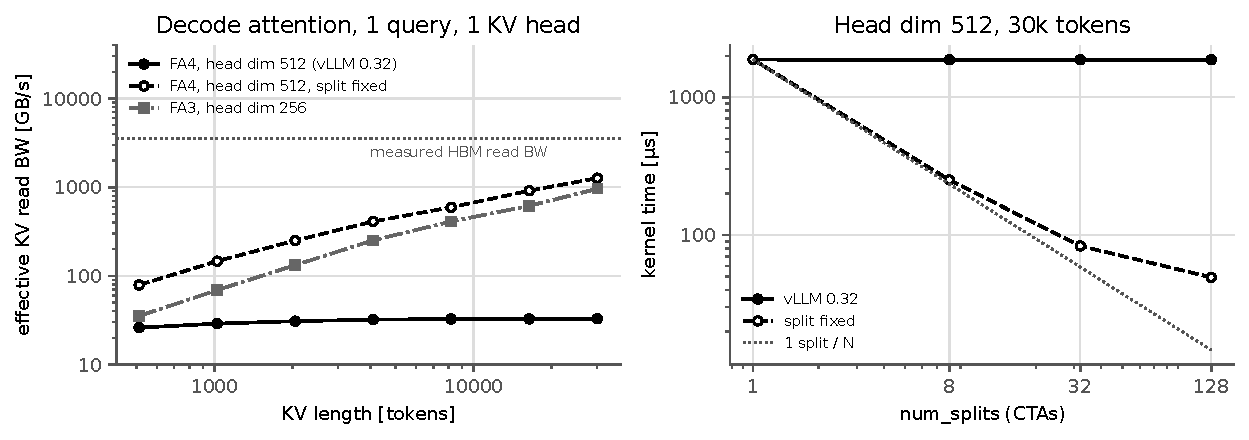
\includegraphics[width=\linewidth]{attn_kernel.pdf}
\caption{global 層（head dim 512）の decode Attention カーネル単体の測定（KV ヘッド 1 本，ページサイズ 16，E9）．
左：KV 長と実効帯域．vLLM 0.32.0 の FA4 は KV 長によらず 1 SM 分の帯域（約 33\,GB/s）で頭打ちになる．
右：30k トークンでの split 数と時間．修正前は split 数を増やしても時間が変わらない．点線は 1 split の時間を split 数で割った理想．}
\label{fig:attn-kernel}
\end{figure}

\paragraph{Attention backend を替えると decode は速くなるが，prefill は遅くなる．}
バグを特定する前に，原因がこのカーネルにあることを確かめるため，同じモデルを Triton の Attention backend（\texttt{-{}-attention-backend TRITON\_ATTN}）で測り直した（E8，表\ref{tab:backend}）．
30k での TPOT は E2B で 17.0\,ms から 6.7\,ms（2.5 倍速），31B で 40.7\,ms から 27.5\,ms（1.5 倍速）に縮んだ．
一方で 32k の TTFT は E2B で 1.9 倍，31B で 1.65 倍に伸びる．prefill では FA4 の方が Triton より速いからである．
FP8 の KV キャッシュでは local 層が FA3 に替わるが，31B の 30k での TPOT は 41.0\,ms で変わらなかった．時間の大半を占める global 層が FA4 のままだからである
（E2B は FP8 KV キャッシュでは CUDA Graph の取り込み中にエラーとなり，起動しなかった）．

\subsection{split-KV を修正した FA4 での測り直し}
\label{sec:ctx-fix}
修正の効果をサービング全体で確かめるため，1 行の修正を入れた FA4 で E1 の単一ストリーム計測と E6 の長いコンテキストのプロファイルを測り直した（E9）．
インストールした vLLM 自体は書き換えておらず，計測用のサーバプロセスの中でだけ，範囲を計算する関数を修正版に差し替えている．
それ以外の条件（モデル，オプション，ワークロード）は元の計測と同じである．

\begin{itemize}
\item \textbf{長いコンテキストの decode の遅さはほぼ消えた．}30k での TPOT は E2B で 17.0\,ms から 3.7\,ms（4.6 倍速），31B で 40.7\,ms から 23.3\,ms（1.7 倍速）になった（表\ref{tab:ctx}，\ref{tab:backend}）．
      TPOT の増分は 0.1--1.3\,ms で，KV 読み出しの理論増分の 0.8--1.8 倍に収まり，Qwen3 と同じ水準になった．
\item \textbf{カーネル 1 回の時間は 16--42 倍短くなった．}global 層 1 回は E2B で 1.84\,ms から 44\,µs，31B で 1.57\,ms から 98\,µs になり（combine を含む），実効帯域は 1.4--2.2\,TB/s に上がった（表\ref{tab:attn-bw}）．
      E2B の 30k での decode 1 ステップに Attention が占める割合は 81\% から 17\% に下がった．
\item \textbf{短いコンテキストの decode も 0.6--1.0\,ms 速くなった．}local 層のカーネルも 128 split のうち 1 個しか働いていなかったからで，E2B の local 層 1 回は 26\,µs から 15\,µs になった．
\item \textbf{prefill と精度は変わらない．}TTFT の差は 32k で $+2$--$6\%$ にとどまり，Babilong の正答数も同じだった（E2B のみ 36 問中 16 問から 15 問）．
      split の部分結果をまとめる順序が変わるため，BF16 の丸めの違いで greedy 生成の出力が途中から分かれるリクエストはある．
\item \textbf{Triton backend より decode も prefill も速い．}修正後の FA4 は 30k の TPOT で Triton を E2B で 1.8 倍，31B で 1.2 倍上回る．
      Triton で decode が速くなったのは Triton が速いからではなく，FA4 が壊れていたからである．
\item \textbf{高並列のスループットは変わらない．}31B の同時実行スイープ（E2）でも，修正後の出力スループットは 32 並列で 507\,tok/s，64 並列で 494\,tok/s で，修正前（533，522\,tok/s）と同程度だった．
      SWE-bench のプロンプトは 1.3k トークン程度と短く，global 層の Attention が時間に占める割合が小さいからで，\S\ref{sec:conc} の頭打ちの原因はこのバグではない．
\end{itemize}

\begin{table}[htbp]\centering\small
\caption{Attention backend と KV キャッシュの型による TPOT と TTFT の違い（ms，中央値）．TPOT（<1k）は 1k トークン未満のプロンプト，$\sim$30k と TTFT は Babilong の各長さ設定（32k 設定は約 31k トークン）．}
\label{tab:backend}
\begin{tabular}{llrrrr}\toprule
モデル & Attention backend & TPOT（<1k） & TPOT（$\sim$30k） & TTFT（8k） & TTFT（32k） \\\midrule
Gemma4 E2B & FA4（既定） & 4.20 & 16.96 & 105 & 602 \\
Gemma4 E2B & Triton & 3.51 & 6.73 & 150 & 1{,}122 \\
Gemma4 E2B & FA4（split-KV 修正後） & 3.59 & 3.70 & 108 & 613 \\
Gemma4 31B & FA4（既定） & 23.01 & 40.66 & 1{,}167 & 5{,}999 \\
Gemma4 31B & Triton & 21.85 & 27.53 & 1{,}529 & 9{,}915 \\
Gemma4 31B & FA3/FA4（FP8 KV） & 23.04 & 40.99 & 1{,}214 & 6{,}185 \\
Gemma4 31B & FA4（split-KV 修正後） & 22.02 & 23.27 & 1{,}225 & 6{,}309 \\
Qwen3-32B & FA3（既定） & 22.00 & 24.93 & 1{,}290 & 7{,}179 \\\bottomrule
\end{tabular}
\end{table}

\textbf{アーキテクチャ上は Gemma~4 の方が長いコンテキストの decode に有利}（30k での KV 読み出しは同クラスの Qwen3 の 28--42\%）であり，
修正後はその利点がそのまま表れる．30k での TPOT は 31B が 23.3\,ms で Qwen3-32B（24.9\,ms）より 7\% 速く，26B-A4B が 4.9\,ms で Qwen3-30B-A3B（5.5\,ms）より 12\% 速い．
vLLM 0.32.0 での「Gemma~4 は長いコンテキストの decode が遅い」という結果は，モデルではなくこのバグによるものだった．

\begin{keybox}{コラム：upstream にコミットするチャンスは，すでに過ぎていた}
このバグを見つけて 1 行の修正で 38 倍速くなったとき，筆者は「これは vLLM にプルリクエストを出せる」と思った．
出力が正しいまま 128 個の CTA のうち 1 個しか働かないという，テストでは見つからない種類のバグであり，Gemma~4 の長いコンテキストの decode を 4.6 倍速くする．
ところが最新の upstream を調べると，すでに直っていた．

\begin{itemize}
\item FA4 のカーネルは vLLM のリポジトリには含まれておらず，ビルド時に vllm-project/flash-attention の特定のコミットを取り込んでいる．
\item そのリポジトリでは 2026 年 9 月 28 日に \textit{Fix SM90 SplitKV block range partitioning}（\#198）として，本書の修正と同じ 1 行の修正がマージされていた．
\item vLLM 側では 10 月 13 日のコミット（\#55866）で取り込むコミットが \texttt{9cd61de} から \texttt{b273a02} に更新され，v0.32.1rc0 以降（v0.33.0rc0/rc1 と main）には修正が入っている．
      このコミットには，head dim 512 の forward の shared memory の競合を直す修正（\#203）も含まれている．
\item 本書で使った v0.32.0 は 10 月 17 日のリリースで，main への修正より後に出ているが，リリース用のブランチには修正が入っておらず，修正前のコミットを取り込んでいる．
      執筆時点で修正を含むのは候補版（rc）だけで，正式リリースの最新版である v0.32.0 を使う利用者はこのバグの影響を受ける．
\end{itemize}

コミットのチャンスだと思ったのにすでに直っていて，正直なところ悔しい．
それでも，このバグがハードウェアの上で何を起こしていたか（1 SM しか働かず，HBM 帯域の 1\% で動いていた）と，修正でサービング性能がどれだけ変わるか（表\ref{tab:ctx}）を定量的に示した報告は，筆者の調べた範囲では見つからなかった．
v0.32.0 で Gemma~4 を長いコンテキストで動かしている場合は，修正を含む版（v0.32.1rc0 以降）に上げれば decode が最大 4.6 倍速くなる．
\end{keybox}

%---------------------------------------------------------------------
\subsection{同時実行：バッチによる償却と，MoE・KV 容量の限界}
\label{sec:conc}
同時実行数スイープ（E2）では，SWE-bench Lite のプロンプト（平均約 1.3k トークン）を出力 256 トークン固定で流した．

\paragraph{バッチで重みの読み出しを償却できる．}
E2B のスループットは同時実行 1 の 189\,tok/s から 64 の 6{,}869\,tok/s（36 倍）まで伸び，TPOT は 4.4\,ms から 7.7\,ms にしか悪化しない（図\ref{fig:conc-scaling} 左）．
重みはバッチ全体で 1 回しか読まないからである．
64 並列でも dense の arithmetic intensity は 30--50\,FLOP/byte で ridge point（138--214）に届かず，decode はまだ帯域律速の領域にある（同右）．
MoE の 2 モデルは 64 並列でも 7--8\,FLOP/byte にとどまる．バッチを大きくすると読む expert も増えるので，FLOPs と読み出しバイトが一緒に増え，比があまり上がらないためである（\S\ref{sec:moe-load}）．

\begin{figure}[htbp]\centering
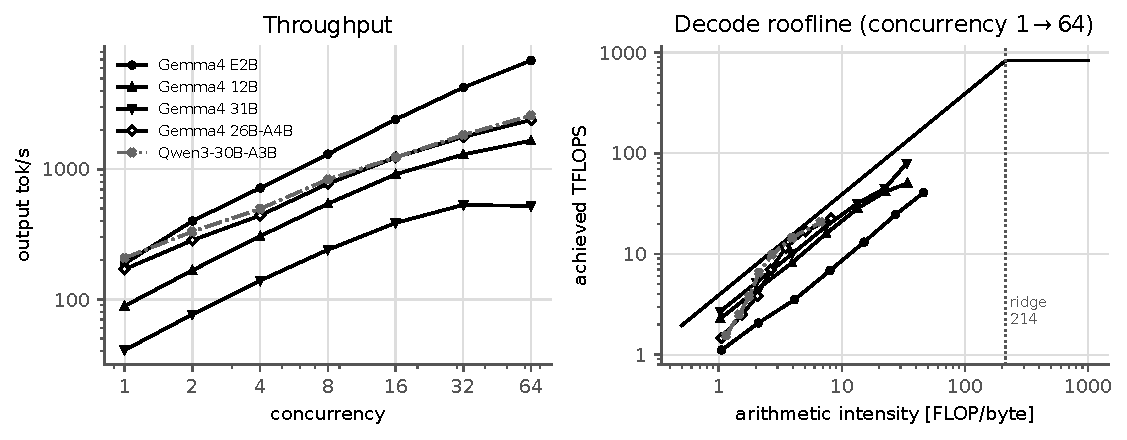
\includegraphics[width=\linewidth]{conc_scaling.pdf}
\caption{同時実行数に対するスループット（左）と，decode ステップのroofline上の位置（右，arithmetic intensityは理論 FLOPs / 理論バイト，到達性能は理論 FLOPs / 実測 TPOT）．dense 3 モデルと MoE 2 モデル．}
\label{fig:conc-scaling}
\end{figure}

\paragraph{高負荷では prefill の計算が TPOT を押し上げる．}
12B の TPOT は 64 並列で 31.6\,ms で，decode だけのroofline下限（11.8\,ms）の 2.7 倍である（図\ref{fig:conc-prefill}）．
chunked prefill では，定常状態で出力 1 トークンあたり約 5 トークン分の新規リクエストの prefill が同じステップに入る．
その計算時間（実測 GEMM ピーク 492\,TFLOPS で 18.0\,ms，514\,TFLOPS なら 17.2\,ms）を，HBM の読み出し時間（11.8\,ms）と重ならずに足し合わせた見積もり（破線，492\,TFLOPS の場合）は 29.0--29.9\,ms になり，
同時実行数による TPOT の増え方をよく再現する．
同時実行 1 でも残る約 4.5\,ms の差は，\S\ref{sec:short} で見た固定的な latencyである．
入力が長く出力が短いワークロードほどこの影響は大きく，prefill/decode の分離や \texttt{max-num-batched-tokens} の調整が効く領域である．

\begin{figure}[htbp]\centering
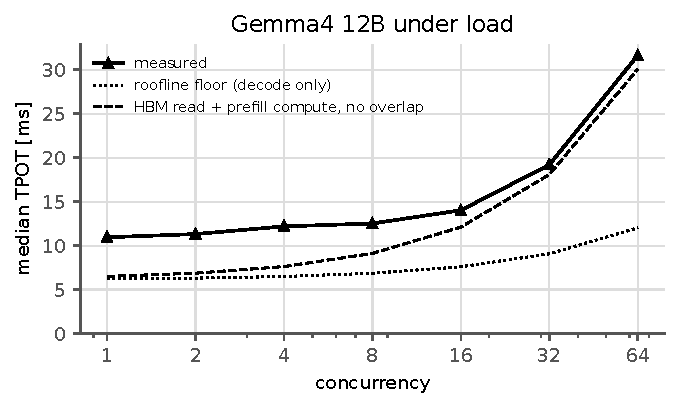
\includegraphics[width=0.6\linewidth]{conc_prefill.pdf}
\caption{12B の TPOT と同時実行数．点線は decode だけのroofline下限，破線は HBM 読み出しと prefill の計算が重ならないとした見積もり．}
\label{fig:conc-prefill}
\end{figure}

\paragraph{MoE の「アクティブ 3.8B」は単一ストリームでのみ成り立つ．}
\label{sec:moe-load}
26B-A4B の TPOT は 5.7\,ms から 23.7\,ms へと急に悪化し，64 並列では dense の 12B に近づく（図\ref{fig:conc-moe}）．
式\eqref{eq:bytes}の $f(B)$ により，1 ステップで読む重みが $B=1$ の 7.7\,GB から $B=64$ で 50\,GB まで増え，12B（24\,GB）の 2 倍になるからである
（expert が等確率・独立に選ばれると仮定した理論値．偏りがあれば実際はこれより少ない）．
Qwen3-30B-A3B も同じ挙動で，最大スループットは 26B-A4B が 2{,}392\,tok/s，Qwen3-30B-A3B が 2{,}599\,tok/s とほぼ同じである．

\begin{figure}[htbp]\centering
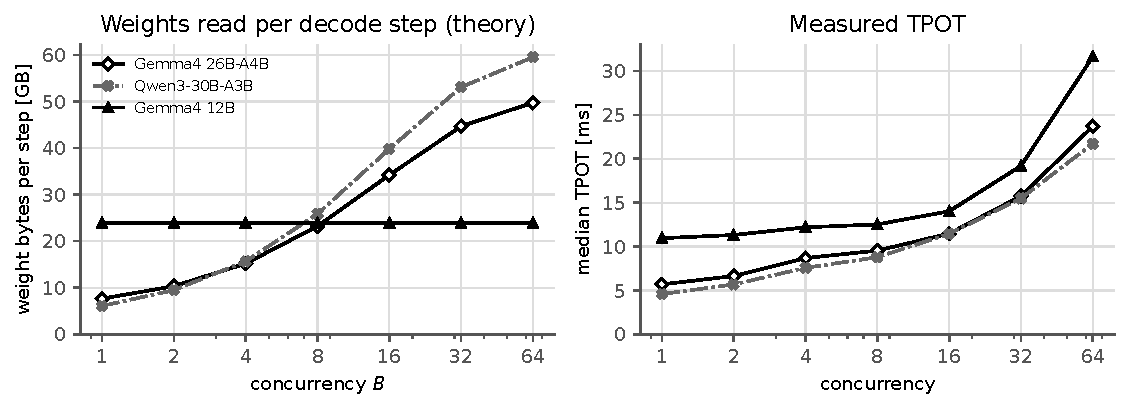
\includegraphics[width=\linewidth]{conc_moe.pdf}
\caption{MoE 2 モデルと dense の 12B について，1 ステップで読む重みの理論値（左，expert が等確率・独立に選ばれると仮定）と実測 TPOT（右）．}
\label{fig:conc-moe}
\end{figure}

\paragraph{31B は 32 並列で頭打ちになり，KV が足りなくなる．}
31B は 32 並列の 533\,tok/s から伸びが止まり，64 並列では TTFT が 18\,s に跳ね上がる（図\ref{fig:conc-kv}）．
サーバログでは KV キャッシュ使用率が 98.6\%，同時に実行されたリクエストは最大 36 本で，残りは待ち行列に入っていた．
重みを載せた後の KV 領域は 27\,GiB しかない．さらに約 1.8k トークンのリクエストはwindow size（1024）を超えて local 層が満杯になるため，1 トークンあたり平均の KV が Qwen3-32B の 2.1 倍（535 対 256\,KiB）になる（図\ref{fig:kv}）．
その結果，64 並列では Qwen3-32B（839\,tok/s）が 31B を 1.6 倍上回った．

\paragraph{FP8 KV キャッシュで容量を倍にしても，スループットは伸びない．}
KV 容量がスループットを決めているのかを確かめるため，31B を FP8 の KV キャッシュで同じ条件で測った（E8）．
KV 領域は 59{,}026 トークンから 114{,}656 トークン（1.94 倍）に増え，64 並列でも 64 本すべてが同時に走るようになった．
その結果 64 並列の TTFT は 18.2\,s から 4.4\,s に縮んだが，TPOT は 52\,ms から 91\,ms に伸び，出力スループットは 522\,tok/s から 527\,tok/s とほとんど変わらなかった．
同時に走るリクエストが最大 36 本から 64 本に増えた分だけ 1 ステップが長くなり，相殺されたのである．
8--32 並列では FP8 KV の方がむしろ 5--9\% 低い（32 並列で 487 対 533\,tok/s）．KV を FP8 に変換する処理や層ごとの backend 切り替えの上乗せと考えられるが，本書では分解していない．
入力を含めた処理トークン数は，64 並列で 31B が約 3{,}000\,tok/s，Qwen3-32B が約 4{,}300\,tok/s である．パラメータ数はほぼ同じなので，31B は 1 トークンを処理する効率そのものが 3 割低い．
したがって \textbf{31B の高並列スループットの頭打ちは KV 容量ではなく，1 ステップの処理の効率で決まっている}．
KV の不足は待ち行列を生んで TTFT を悪化させるが，スループットの上限は決めていない．
\S\ref{sec:ctx} の split-KV のバグを修正してもスループットは変わらなかったので（\S\ref{sec:ctx-fix}），このバグは原因ではない．どのカーネルが効率を下げているかは，本書では分解していない．

\begin{figure}[htbp]\centering
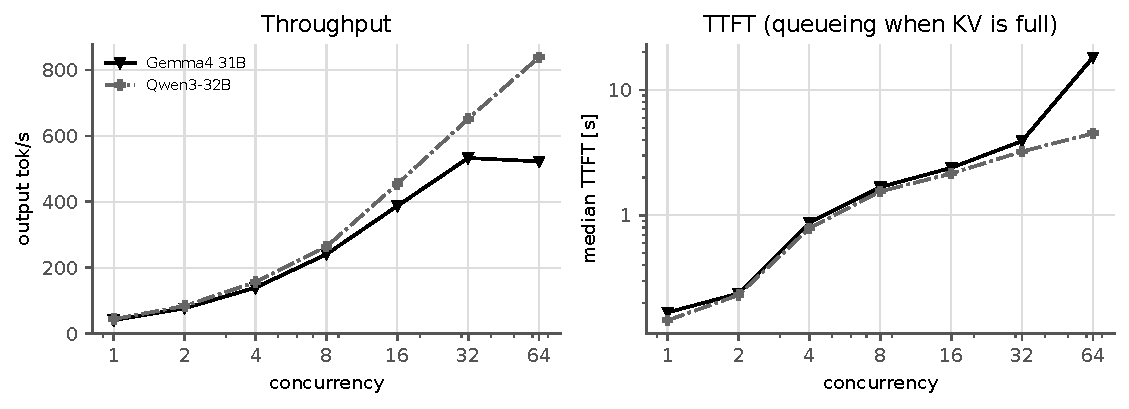
\includegraphics[width=\linewidth]{conc_kv.pdf}
\caption{31B と Qwen3-32B のスループット（左）と TTFT（右）．31B は 32 並列を超えると KV が足りず，リクエストが待ち行列に入る．}
\label{fig:conc-kv}
\end{figure}

\paragraph{vLLM の KV 割り当て（E4）．}
Qwen3 では vLLM が見積もる最大同時実行数が理論値と一致するが，Gemma~4 の 12B/26B/31B では理論値の 1/4--1/6 しか確保されていない（表\ref{tab:kvcap}）．
31B で最大長 32{,}768 の起動に必要と報告された 27.5\,GiB は，全層をフルコンテキストとした場合の理論値（27.50\,GiB）と一致しており，
少なくとも起動時のメモリ見積もりは sliding window の分を差し引いていない．
運用中の割り当てでも，local 層（head dim 256，KV ヘッド 8--16）と global 層（head dim 512，KV ヘッド 1--4）でページの大きさを揃えるためのパディングが理論値との差を生んでいると考えられるが，本書では確認していない．

\begin{table}[htbp]\centering\small
\caption{vLLM が確保する KV 領域と，最大長リクエストの最大同時実行数．ideal は窓と KV 共有を考慮した理論 KV 量（K と V を両方格納）で割った値，no window は全層をフルコンテキストとした場合．}
\label{tab:kvcap}
\begin{adjustbox}{max width=\linewidth}
\begin{tabular}{lrrrrrr}
\toprule
Model & KV pool [GiB] & req. len & ideal KV/req [GiB] & max conc. (vLLM) & max conc. (ideal) & max conc. (no window) \\
\midrule
Gemma4 E2B & 74.2 & 40k & 0.24 & 173.2 & 309 & 105.5 \\
Gemma4 E4B & 68.8 & 40k & 0.64 & 54.2 & 107 & 31.5 \\
Gemma4 12B & 61.0 & 40k & 0.94 & 10.3 & 65 & 4.6 \\
Gemma4 26B-A4B & 35.1 & 40k & 0.98 & 8.6 & 36 & 4.1 \\
Gemma4 31B & 27.0 & 34k & 3.44 & 1.7 & 8 & 0.9 \\
Qwen3-30B-A3B & 27.1 & 40k & 3.75 & 7.2 & 7 & 7.2 \\
Qwen3-32B & 24.8 & 40k & 10.00 & 2.5 & 2 & 2.5 \\
\bottomrule
\end{tabular}

\end{adjustbox}
\end{table}

%---------------------------------------------------------------------
\subsection{MTP Drafter によるspeculative decoding}
\label{sec:mtp}
\begin{table}[htbp]\centering\small
\caption{speculative decodingの方式・draft length別のmean acceptance length AL と TPOT 高速化（中央値）．n-gram はプロンプト内の n-gram 照合（モデル不要）．
Babilong* は出力長を固定するため EOS を抑制しており，回答後に同じ文を繰り返す（acceptance rateが高く出る）ので参考値．}
\label{tab:spec}
\begin{adjustbox}{max width=\linewidth}
\begin{tabular}{llrrrrrr}
\toprule
Model & method & Synthetic AL & Synthetic speedup & SWE-bench AL & SWE-bench speedup & Babilong* AL & Babilong* speedup \\
\midrule
Gemma4 E2B & MTP $\gamma$=1 & 1.63 & 1.46$\times$ & 1.81 & 1.66$\times$ & 1.66 & 1.47$\times$ \\
Gemma4 E2B & MTP $\gamma$=2 & 1.96 & 1.59$\times$ & 2.42 & 2.05$\times$ & 2.07 & 1.62$\times$ \\
Gemma4 E2B & MTP $\gamma$=4 & 2.28 & 1.58$\times$ & 3.22 & 2.37$\times$ & 2.67 & 1.75$\times$ \\
Gemma4 E2B & MTP $\gamma$=8 & 2.46 & 1.33$\times$ & 4.10 & 2.28$\times$ & 3.08 & 1.48$\times$ \\
Gemma4 E4B & MTP $\gamma$=4 & 2.43 & 1.78$\times$ & 3.32 & 2.66$\times$ & 2.19 & 1.60$\times$ \\
Gemma4 12B & MTP $\gamma$=4 & 2.71 & 1.63$\times$ & 3.63 & 1.98$\times$ & 3.41 & 2.15$\times$ \\
Gemma4 26B-A4B & MTP $\gamma$=1 & 1.83 & 1.15$\times$ & 1.85 & 1.03$\times$ & 1.80 & 1.24$\times$ \\
Gemma4 26B-A4B & MTP $\gamma$=2 & 2.45 & 1.28$\times$ & 2.55 & 1.16$\times$ & 2.42 & 1.40$\times$ \\
Gemma4 26B-A4B & MTP $\gamma$=4 & 3.31 & 1.43$\times$ & 3.59 & 1.30$\times$ & 3.24 & 1.37$\times$ \\
Gemma4 26B-A4B & MTP $\gamma$=8 & 4.01 & 1.20$\times$ & 4.58 & 1.15$\times$ & 4.08 & 1.18$\times$ \\
Gemma4 31B & MTP $\gamma$=1 & 1.86 & 1.77$\times$ & 1.86 & 1.79$\times$ & 1.89 & 1.80$\times$ \\
Gemma4 31B & MTP $\gamma$=2 & 2.49 & 2.27$\times$ & 2.57 & 2.37$\times$ & 2.68 & 2.50$\times$ \\
Gemma4 31B & MTP $\gamma$=4 & 3.54 & 3.01$\times$ & 3.61 & 3.14$\times$ & 3.98 & 3.55$\times$ \\
Gemma4 31B & MTP $\gamma$=8 & 4.27 & 3.14$\times$ & 4.55 & 3.59$\times$ & 5.86 & 4.79$\times$ \\
Gemma4 31B & n-gram $\gamma$=4 & 1.03 & 0.95$\times$ & 1.42 & 1.32$\times$ & 3.31 & 3.32$\times$ \\
\bottomrule
\end{tabular}

\end{adjustbox}
\end{table}

\paragraph{AL は似ているのに，高速化は大きく違う．}
$\gamma=4$ の TPOT 高速化は 31B 3.08 倍，E4B 2.17 倍，E2B 1.94 倍，12B 1.85 倍，26B-A4B 1.35 倍である（図\ref{fig:mtp}，Synthetic + SWE-bench）．
31B は vLLM PR の報告（$\gamma=8$ で 3.19 倍）とよく一致する．
一方 AL は 2.8--3.6 トークンとモデル間の差が小さく，26B-A4B は 2 番目に高い．
つまり 26B-A4B が効きにくいのは drafter の予測が外れるからではなく，1 ステップのコスト $c$ が大きいからである（後述）．

\begin{figure}[htbp]\centering
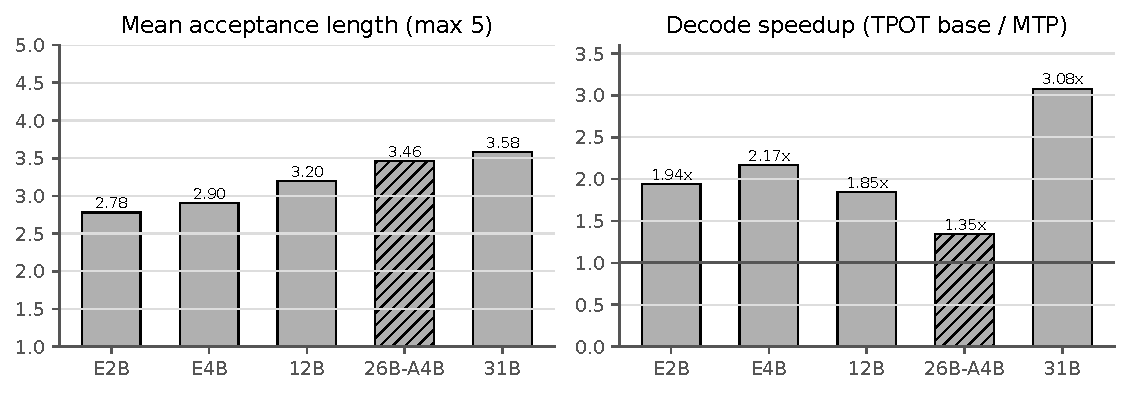
\includegraphics[width=\linewidth]{mtp_speedup.pdf}
\caption{MTP（$\gamma=4$，同時実行 1，Synthetic + SWE-bench）のmean acceptance length（左）と TPOT 高速化（右）．斜線は MoE の 26B-A4B．}
\label{fig:mtp}
\end{figure}

\paragraph{生成内容への依存．}
コードのパッチ生成（SWE-bench）は自然文（Synthetic）より AL が高い（E2B で 3.22 対 2.28）．差分の文脈行はコードのコピーで予測しやすいためである．
リポジトリ別では sympy が最も低く，matplotlib が最も高い（付録の図\ref{fig:genre}）．
モデル不要の n-gram（31B，$\gamma=4$）は，プロンプトからのコピーが多い SWE-bench で 1.32 倍，繰り返しの多い Babilong* で 3.32 倍だが，自由な文章では 0.95 倍とかえって遅くなる（図\ref{fig:mtp-ngram}）．
MTP はどのワークロードでも 3.0--3.5 倍を出しており，\textbf{学習済み drafter の強みは内容によらないacceptance rateにある}．

\begin{figure}[htbp]\centering
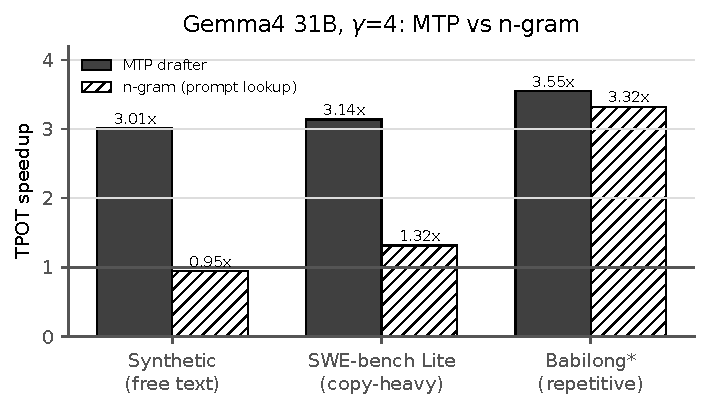
\includegraphics[width=0.62\linewidth]{mtp_vs_ngram.pdf}
\caption{31B（$\gamma=4$）での MTP と n-gram の TPOT 高速化．Babilong* は回答後に同じ文を繰り返すので参考値．}
\label{fig:mtp-ngram}
\end{figure}

\begin{figure}[htbp]\centering
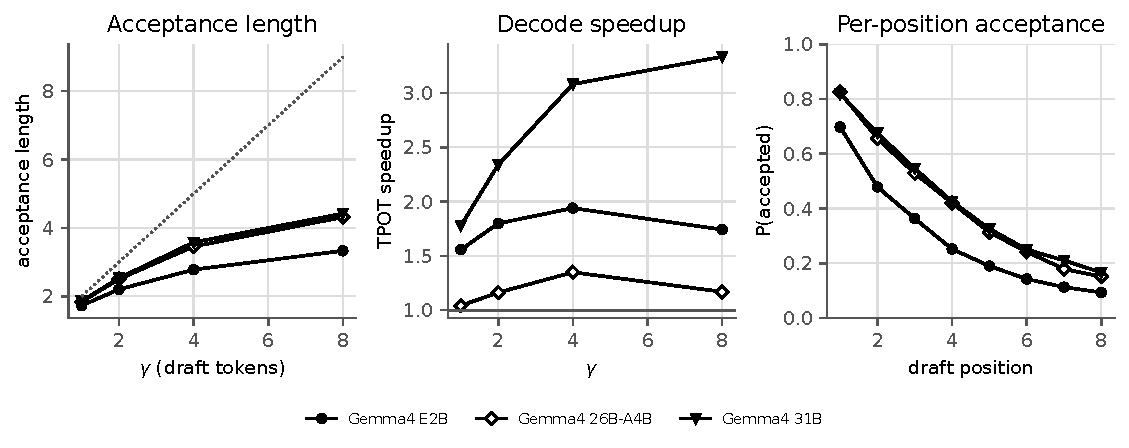
\includegraphics[width=\linewidth]{mtp_gamma.pdf}
\caption{draft length $\gamma$ の影響（Synthetic + SWE-bench）．左：AL（点線は全 acceptの上限 $\gamma+1$），中：TPOT 高速化，右：$\gamma=8$ での位置ごとのacceptance rate．}
\label{fig:gamma}
\end{figure}

\paragraph{なぜ 26B-A4B では効きにくいか：コストモデルによる説明．}
式\eqref{eq:spec}の AL と $c$ を分けると（図\ref{fig:costmodel}），26B-A4B の AL（3.46）は 31B（3.58）とほぼ同じで，差は $c$ にある．
26B-A4B は $\gamma=4$ のverifyで 5 トークン分の expert（一様・独立の仮定で 27.5\%．$B=1$ では 6.3\%）を読むので，verifyだけで通常ステップの 2.3 倍のバイトを読む．
drafter（target の 11\%）4 回分を足すと式\eqref{eq:cpred}で $c_\text{pred}=2.78$ となり，実測の $c=2.56$ と近い．
一方 31B は dense なのでverifyがほぼ無料で，$c_\text{pred}=1.12$（実測 1.16），予測高速化 3.20 倍（実測 3.08 倍）とよく一致する．

E2B/E4B/12B は実測の $c$ が予測より 0.3--0.5 大きい．
E2B/E4B は 1 ステップが 2--4\,ms と短く，drafter 1 回分の固定latencyが相対的に重い．そのため E2B は $\gamma=8$ で $\gamma=4$ より遅くなる．
12B と 26B-A4B では MTP 有効時に GPU が約 50\% の時間idleになっていた（図\ref{fig:nsys-mtp}）．
26B-A4B は別の日に測り直しても，高速化が $\gamma=4$ で 1.41 倍，$\gamma=8$ で 1.24 倍，GPU busy が 48\%（通常の decode は 92\%，31B の MTP は 90\%）で，同じ結果になった（E8）．
drafter の経路で 1 出力トークンあたり CUDA Graph 起動が 12--20 回，通常のカーネル起動が 86--114 回発生しており（通常の decode ではそれぞれ 1.1 回と 25 回），CPU が律速になっている．
drafter の経路を完全に CUDA Graph 化できれば，12B の高速化は 1.85 倍から予測値の 2.7 倍に近づく．
\textbf{最適な $\gamma$ は，大きい dense モデルで 8 以上，小さいモデルで 4 前後，MoE で 4（低負荷時）である．}

\begin{figure}[htbp]\centering
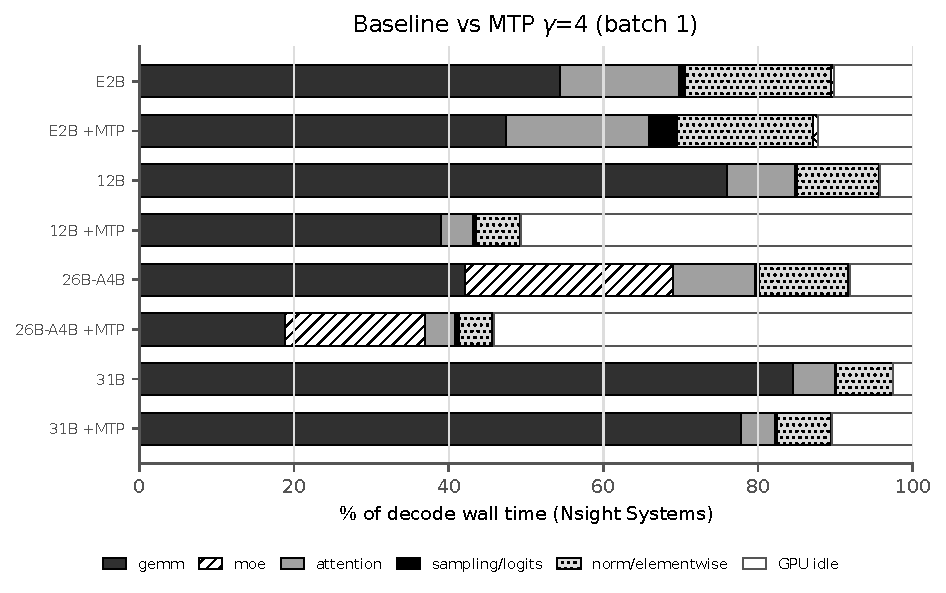
\includegraphics[width=0.85\linewidth]{nsys_mtp.pdf}
\caption{通常の decode と MTP（$\gamma=4$）の時間内訳（Nsight Systems，バッチ 1）．12B と 26B-A4B では MTP 有効時に GPU のidle（白）が約半分を占める．}
\label{fig:nsys-mtp}
\end{figure}

\begin{figure}[htbp]\centering
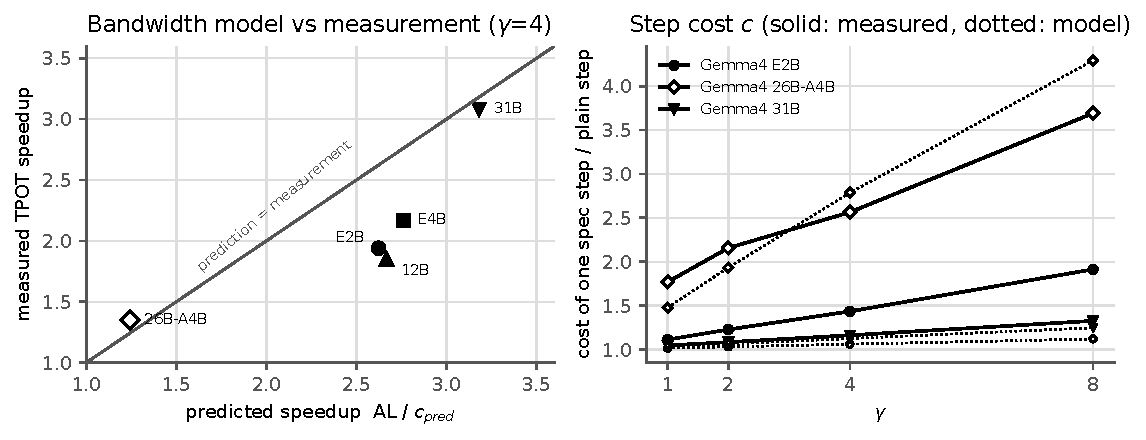
\includegraphics[width=\linewidth]{mtp_cost_model.pdf}
\caption{帯域コストモデルによる予測高速化 AL/$c_\text{pred}$ と実測（左，$\gamma=4$）．$\gamma$ を振った 3 モデルの 1 speculative stepのコスト $c$（右，実線：実測 AL/高速化，点線：式\eqref{eq:cpred}）．}
\label{fig:costmodel}
\end{figure}

\paragraph{高負荷時の MTP．}
同時実行数を上げると dense モデルの MTP の利得は縮む（図\ref{fig:mtp-load}）．E2B では同時実行 1 の 2.3 倍が 64 では 1.16 倍になる．
バッチが大きくなるとarithmetic intensityが上がり，verifyトークン分の計算が無料ではなくなるためである．
逆に 26B-A4B は 1.25 倍から 1.51 倍へと利得が\emph{増える}．高負荷ではもともと expert の大半を読んでいるので，verifyトークンを増やしても読み出しバイトがほとんど増えないからである．
vLLM PR が報告した「26B-A4B では MTP の利得がバッチとともに増える」傾向と一致する．

\begin{figure}[htbp]\centering
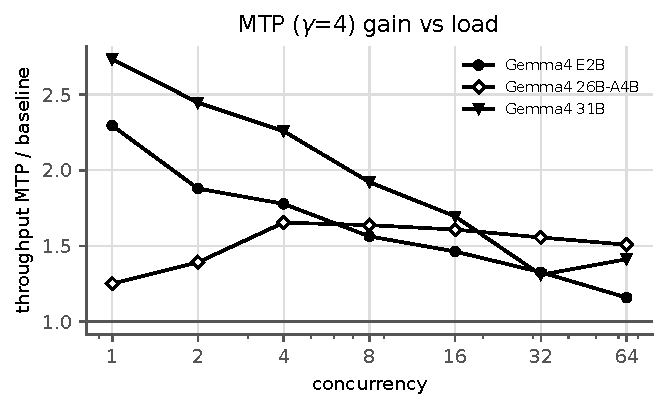
\includegraphics[width=0.6\linewidth]{concurrency_mtp.pdf}
\caption{同時実行数ごとの MTP（$\gamma=4$）のスループット向上率（条件は図\ref{fig:conc-scaling} と同じ）．dense の E2B・31B と MoE の 26B-A4B で傾向が逆になる．}
\label{fig:mtp-load}
\end{figure}

%=====================================================================
\section{外部の結果との比較と総合評価}
\label{sec:discussion}

\subsection{外部の結果と整合しているか}
本書の数値を，vLLM の Gemma~4 MTP 実装 PR\cite{vllmpr}，第三者による H100 でのベンチマーク\cite{jarvislabs,inferencebench}，Google の MTP 紹介記事\cite{mtpblog}と比べた（表\ref{tab:external}）．
外部の測定は GPU（H100 SXM），vLLM のバージョン，Attention backend，ワークロードが本書と異なるので，比べられるのは傾向と桁である．

\begin{table}[htbp]\centering\small
\caption{外部の結果との比較（同時実行 1 は出力 tok/s，括弧内は baseline に対する倍率）．
外部の測定はいずれも H100 SXM（HBM 3.35\,TB/s）と SPEED-Bench を使っており，jarvislabs は Attention backend に Triton を使っている．}
\label{tab:external}
\begin{adjustbox}{max width=\linewidth}
\begin{tabular}{lllll}\toprule
指標 & 本書（H100 NVL，vLLM 0.32） & vLLM PR\cite{vllmpr} & jarvislabs\cite{jarvislabs} & 整合 \\\midrule
31B baseline，同時実行 1 & 42\,tok/s（TPOT 23.6\,ms） & 42.6\,tok/s & 40.3\,tok/s（TPOT 24.4\,ms） & ○ \\
31B MTP $\gamma=8$，同時実行 1 & 148\,tok/s（3.33$\times$） & 136\,tok/s（3.19$\times$） & 125\,tok/s（3.11$\times$） & ○ \\
31B baseline，同時実行 16 & 387\,tok/s（TPOT 32.2\,ms） & -- & 375\,tok/s（TPOT 32.9\,ms） & ○ \\
26B-A4B baseline，同時実行 1 & 175\,tok/s & 169\,tok/s & 177\,tok/s & ○ \\
26B-A4B MTP，同時実行 1 & 226\,tok/s（1.35$\times$，$\gamma=4$） & 270\,tok/s（1.60$\times$，$\gamma=4$） & 264\,tok/s（1.49$\times$，$\gamma=8$） & △ 本書が低い（再計測でも 1.41$\times$） \\
26B-A4B の MTP 利得と負荷 & 1.25$\to$1.51$\times$（同時実行 1$\to$64） & 1.60$\to$2.27$\times$（バッチ 1$\to$64） & -- & ○ 同じ傾向 \\
E4B MTP $\gamma=4$，同時実行 1 & 2.17$\times$ & 1.78$\times$ & -- & △ 本書が高い \\
\bottomrule\end{tabular}
\end{adjustbox}
\end{table}

\begin{itemize}
\item \textbf{31B の baseline と MTP はよく一致する．}baseline の出力速度は 3 つの測定で 40--43\,tok/s，MTP の高速化は 3.1--3.3 倍にそろう．
      同時実行 16 での TPOT も 32--33\,ms で一致する．
      H100 NVL の HBM 帯域は SXM より 16\% 大きいが，31B の baseline はほぼ同じである．重みの読み出しから求めた実効帯域はどちらも約 2.6\,TB/s で，理論帯域に対しては本書が 67\%，SXM が 78\% になる．
      帯域の大きい NVL でも，実際に引き出せる帯域の絶対値は SXM と変わらないことを示唆している．
\item \textbf{26B-A4B の MoE で MTP が効きにくいことも共通している．}Google の記事も 26B の MoE はバッチ 1 で routing が難しく，バッチを増やすと利得が増えると述べており\cite{mtpblog}，vLLM PR の表も同じ傾向を示す．
      これは \S\ref{sec:mtp} のコストモデル（verify で読む expert が増える）と整合する．
      ただし本書の高速化（1.35 倍）は外部（1.49--1.60 倍）より低い．baseline はほぼ同じなので，差は MTP 側にある．
      測り直しても 1.41 倍で外部より低く，baseline の TPOT も $\pm 2\%$ で一致したので，測定のばらつきではない．
      本書では 26B-A4B の MTP 有効時に GPU が約半分 idle になっており（図\ref{fig:nsys-mtp}，再計測でも GPU busy 48\%），CPU 側の処理が律速していた．
      CPU の性能や vLLM のバージョンで CUDA Graph 化される範囲が変わるとこの部分が大きく変わるため，それが差の原因と考えられる．
\item \textbf{高負荷のスループットはワークロードの形で大きく変わる．}inferencebench は H100 SXM の 31B で同時実行 32 のとき 855\,tok/s（入力 2048，出力 1024 トークン）を報告しており\cite{inferencebench}，本書の 533\,tok/s（入力 約 1.3k，出力 256 トークン）より高い．
      出力 1 トークンあたりの prefill 量は先方が 2 トークン，本書が 5.2 トークンであり，\S\ref{sec:results} の prefill 混入の議論から，出力が長いほどスループットが高くなるのは整合する．
\item \textbf{長いコンテキストの decode の遅さを定量的に報告した外部の結果は見つからなかった．}
      原因の split-KV のバグは flash-attention 側で 2026 年 9 月に修正済みで（\S\ref{sec:ctx} のコラム），vLLM v0.32.1rc0 以降には入っている．
      また head dim 512 の global 層が Attention backend の選択を難しくしていることはコミュニティでも知られている．
      vLLM には，head dim 混在のため全層で Triton に切り替わり E4B が RTX 4090 で約 9\,tok/s しか出ないという報告\cite{vllmissue38887}や，local 層だけ FlashAttention を使えるようにする PR\cite{vllmpr38891}（2026 年 10 月時点で未マージ）がある．
      jarvislabs が Triton backend で測っているのに対し，本書の vLLM 0.32 は FA4 を選ぶ（コード\ref{lst:fa4}）など，バージョンによって使われるカーネル自体が変わっている．
      本書でも backend を Triton に替えると 30k での TPOT が 1.5--2.5 倍速くなり，prefill が 1.7--1.9 倍遅くなった（表\ref{tab:backend}）．
\end{itemize}

\subsection{Qwen3 と比べて良い結果か}
結論は，\textbf{アーキテクチャとしては Gemma~4 が優れている点が多いが，現在の vLLM の上ではその一部しか性能に表れておらず，条件によっては Qwen3 に負ける}である．

\begin{table}[htbp]\centering\small
\caption{同クラスの Qwen3 に対する Gemma~4 の評価．○：Gemma~4 が良い，△：同等，×：Gemma~4 が悪い．}
\label{tab:verdict}
\begin{tabular}{L{0.25\linewidth}cL{0.34\linewidth}L{0.24\linewidth}}\toprule
観点 & 評価 & 根拠 & 原因 \\\midrule
長いプロンプトの TTFT & ○ & 32k で 16--33\% 短い & Hybrid Attention（設計） \\
単一ストリームの decode（短いコンテキスト） & △ & 31B 22.9 対 22.0\,ms，26B-A4B 5.3 対 4.6\,ms & ほぼパラメータ数どおり \\
MTP を使った単一ストリームの decode & ○ & 31B は 3.1--3.3 倍で Qwen3-32B（baseline）の約 3 倍速い & 公式 drafter（設計） \\
長いコンテキストの decode & \shortstack{×\\{\scriptsize 修正後 ○}} & v0.32.0 では 30k で TPOT の増分が 9--18\,ms（Qwen3 は 1--3\,ms）．split-KV の修正後は 31B 23.3 対 24.9\,ms，26B-A4B 4.9 対 5.5\,ms & FA4 の split-KV のバグ（実装，v0.32.1rc0 で修正） \\
長いコンテキストの KV 量（理論） & ○ & 32k で 31B 3.3\,GiB 対 8.0\,GiB & Hybrid Attention（設計） \\
短いリクエストの高並列スループット & × & 64 並列で 31B は Qwen3-32B の 0.6 倍．FP8 KV で KV 容量を倍にしても変わらない & 1 トークンの処理効率（実装と考えられる） \\
MoE の高負荷スループット & △ & 2{,}392 対 2{,}599\,tok/s & 両者とも expert の読み出しが増える \\
\bottomrule\end{tabular}
\end{table}

表\ref{tab:verdict}で × がついた 2 点のうち，長いコンテキストの decode は完全に実装の問題であり（1 行の修正で消え，修正後は Qwen3 より速い），
高並列のスループットも KV 容量ではなく 1 トークンの処理効率で決まっていた．
つまり Gemma~4 の「残念な」結果の多くは\textbf{ソフトウェアで直せる}種類のものである．
逆に，○の項目のうち MTP による高速化は vLLM ですでに使え，外部の測定でも再現している．
利用者の立場では，現時点で次のように使い分けるのがよい．
\begin{itemize}
\item \textbf{低負荷・低 latency の対話}：31B + MTP（$\gamma=4$--8）が最も速い．同クラスの Qwen3-32B の約 3 倍の速さで出力できる．
\item \textbf{長いプロンプトを読ませる用途}（RAG，要約，長い文脈での対話）：prefill が速く，split-KV の修正後は decode も Qwen3 より速い Gemma~4 が有利である．
      ただし vLLM v0.32.0 では長いコンテキストの decode が 1.7--4.6 倍遅いので，修正を含む v0.32.1rc0 以降を使う．
      v0.32.0 のまま Attention backend を Triton にする回避策は，decode は速くなるが prefill が 1.7--1.9 倍遅くなり，修正版の FA4 にどちらでも劣る．
\item \textbf{短いリクエストを大量にさばく用途}：31B のスループットは 64 並列で Qwen3-32B の 0.6 倍で，FP8 KV キャッシュでも伸びない．
      FP8 KV キャッシュは待ち行列を消して TTFT を 18\,s から 4.4\,s に縮めるので，TTFT を抑えたい場合には有効である．スループットが重要なら Qwen3-32B が有利である．
\end{itemize}

\subsection{コミュニティとして何をすべきか}
本書の測定から，効果が大きいと見積もれる順に挙げる．
\begin{enumerate}
\item \textbf{split-KV の修正を含む版をリリースし，利用者に知らせる．}
      vLLM v0.32.0 の FA4 は split-KV の分割数が渡っておらず，128 個の CTA のうち 1 個しか働かない（\S\ref{sec:ctx}）．
      修正は flash-attention 側にも vLLM の main にもすでに入っているが，執筆時点の正式リリースは修正前の v0.32.0 である．
      修正すると 30k での TPOT は E2B で 17\,ms から 3.7\,ms，31B で 41\,ms から 23\,ms になる（\S\ref{sec:ctx-fix}）．
      出力が正しいまま遅くなる種類のバグはテストで見つからないので，「split 数を増やすと時間が縮む」ことを確かめる性能テストがあれば再発を防げる．
      Triton backend への切り替えや，local 層だけ FA3 を使う層ごとの選択（PR\cite{vllmpr38891}）は，修正版の FA4 があれば不要になる．
\item \textbf{KV キャッシュ管理の改善．}
      起動時の見積もりが sliding window を差し引いていないこと，運用時の割り当てが理論値の 1/4--1/6 にとどまることを直せば，同じメモリでより多くのリクエストを同時に走らせられる．
      ただし FP8 KV キャッシュで容量を倍にした実験では，待ち行列が消えて TTFT は縮んだがスループットは変わらなかった（\S\ref{sec:conc}）．効果は主に TTFT に表れ，スループットを上げるには 1 ステップの処理効率の改善と組み合わせる必要がある．
      さらに K=V の global 層で RoPE 前の K を 1 本だけ保存すれば，global 層の KV を半分にできる．
\item \textbf{drafter 経路の CUDA Graph 化．}
      12B と 26B-A4B では MTP 有効時に GPU が半分 idle で（26B-A4B は再計測でも GPU busy 48\%），CPU からのカーネル起動が律速している．完全に CUDA Graph 化できれば 12B の MTP は 1.85 倍から帯域モデルの予測（2.7 倍）に近づき，26B-A4B も外部の 1.5--1.6 倍に近づくと考えられる．
      負荷に応じて $\gamma$ を自動で変える仕組みも，dense と MoE で最適値が逆向きに動く（\S\ref{sec:mtp}）ことから有用である．
\item \textbf{ベンチマークの報告のしかた．}
      Gemma~4 は vLLM のバージョンによって Attention backend が Triton，FA4 などと変わり，ワークロードの入出力長でスループットも大きく変わる．
      結果を共有するときは，vLLM のバージョン，Attention backend，入力長・出力長，同時実行数を併記することが，比較できる知見を積み上げるうえで重要である．
\end{enumerate}

%=====================================================================
\clearpage
\section{ボトルネックとチューニングの指針}
\label{sec:tuning}
\begin{table}[H]\centering\small
\caption{ボトルネックと対策のまとめ．}
\label{tab:tuning}
\begin{tabular}{L{0.16\linewidth}L{0.16\linewidth}L{0.29\linewidth}L{0.27\linewidth}}\toprule
対象 & 律速要因 & 根拠 & 有効な対策 \\\midrule
小モデル（E2B/E4B）の decode & カーネルの固定latency & 帯域利用率 28--39\%，1 トークン約 600 カーネル & 同時実行数を上げる（64 並列で 36 倍），MTP（1.9--2.2 倍），normalization・residualのカーネル融合 \\
大 dense（31B）の decode & HBM 帯域 & 帯域利用率 70\%，GEMM は実測ピークの 94\% & 重みの量子化（FP8/INT4），MTP $\gamma \ge 4$（3.1--3.3 倍） \\
MoE（26B-A4B） & 負荷により変化 & 高負荷では読む expert が 25B 相当に増える & 低負荷は MTP の効果が小さい．高負荷では MTP が効く（1.5 倍） \\
長いコンテキストの decode & FA4 の split-KV のバグ（v0.32.0） & 理論値の 26--120 倍，128 CTA のうち 1 個だけが働く & 修正を含む v0.32.1rc0 以降を使う（30k で 1.7--4.6 倍速，TTFT は不変） \\
高並列の TPOT & 混入する prefill の計算 & 12B の 64 並列で 31.6\,ms，HBM 読み出し＋prefill 計算の見積もり 29.9\,ms & prefill/decode の分離，\texttt{max-num-batched-tokens} の調整 \\
KV 容量（高並列） & local 層の KV と vLLM の割り当て & 31B は 1.8k トークンのリクエストで平均 535\,KiB/トークン（Qwen3-32B の 2.1 倍），割り当ては理論値の 1/4--1/6．不足すると待ち行列で TTFT が 18\,s に & FP8 KV キャッシュ（TTFT 18$\to$4.4\,s，スループットは不変），FP8 重み，RoPE 前の K を 1 つだけ格納する K=V の活用 \\
Prefill & 電力制限下の GEMM 性能 & 実測 GEMM ピークの 74--84\% & FP8 GEMM（理論 2 倍） \\
\bottomrule\end{tabular}
\end{table}

%=====================================================================
\section{まとめ}
H100~NVL 1 基・vLLM 0.32 で Gemma~4 ファミリのサービング性能を測り，チェックポイントから求めた理論限界と比べた．
4 つの問いへの答えを，結果とその理由の組でまとめる．

\paragraph{Q1：GPU の性能をどこまで出し切れているか．}
\begin{itemize}
\item 31B の decode は HBM 理論帯域の 70\% に達した．これは GEMM が実測帯域ピークの 94\% で重みを読めており，重みの読み出し以外の上乗せ（1 ステップ約 4.6\,ms）が理想時間 17.2\,ms に対して小さいからである．
\item E2B の decode は 28\% にとどまった．これは重みの読み出し以外に，小さな GEMM・normalizationなどのカーネル群・Attention・GPU idleで 1 ステップ約 2.7\,ms かかり，重みを読む理想時間（1.3\,ms）の 2 倍に達するからである．この上乗せはモデルの大きさによらずほぼ一定なので，読むバイトが少ないモデルほど不利になる．
\item MoE の 26B-A4B は 38\% だった．これは expert 1 つあたりの行列が小さく，expert の GEMM が帯域を使い切れないからである．
\item prefill は実測 GEMM ピークの 74--84\% に達した．データシート値に対して 45--49\% にとどまるのは，H100 NVL が 400\,W の電力制限で大きな GEMM のクロックを下げるからである．同じ理由で GEMM ピーク自体も計測ごとに 492--514\,TFLOPS と揺れた．
\end{itemize}

\paragraph{Q2：アーキテクチャ上の工夫は効いているか．}
\begin{itemize}
\item 32k トークンの TTFT は Qwen3 より 16--33\% 短かった．これはHybrid Attentionによって $P^2$ で増えるAttention計算が global 層だけに限られ，Attentionが FLOPs に占める割合が 36\% から 18\% に下がるからである．window size以下では差がなく，効果はAttentionの割合が大きくなる 4k トークン以上で現れる．
\item 一方，vLLM 0.32.0 では，コンテキストを 30k トークンまで伸ばしたときの TPOT の増分が 9--18\,ms で，Qwen3 の 1--3\,ms を大きく上回った（31B は 41\,ms 対 Qwen3-32B の 25\,ms）．これは FA4 カーネルの split-KV に分割数が渡っておらず，128 個の CTA のうち 1 個だけがすべての KV を読んでいたからである．global 層の実効帯域は 33--137\,GB/s で，1 SM 分の帯域しか出ていなかった．1 行の修正で増分は 0.1--1.3\,ms と理論値並みになり，30k での TPOT は 31B が 23.3\,ms，26B-A4B が 4.9\,ms で，同クラスの Qwen3 よりそれぞれ 7\%，12\% 速くなった．この修正はすでに upstream に入っており，v0.32.1rc0 以降で使える．
\item 64 並列では 31B のスループットが Qwen3-32B の 0.6 倍にとどまり，TTFT は 18\,s に達した．TTFT が長いのは，window sizeを超える約 1.8k トークンのリクエストでは local 層の KV が満杯になって 1 トークンあたり平均の KV が Qwen3-32B の 2.1 倍になり，さらに vLLM の KV 割り当てが理論値の 1/4--1/6 にとどまるため，27\,GiB の KV 領域が尽きてリクエストが待たされるからである．
      一方スループットが低いのは KV 容量のためではない．FP8 KV キャッシュで KV 領域を 1.94 倍にすると TTFT は 4.4\,s に縮んだが，スループットは 522 から 527\,tok/s で変わらなかったからである．
\item 26B-A4B の TPOT は同時実行 1 から 64 で 4 倍に悪化した．これはバッチ内のトークンが別々の expert を選ぶため，1 ステップで読む重みが 7.7\,GB から 50\,GB に増えるからである．
\end{itemize}

\paragraph{Q3：MTP Drafter はどの条件でどれだけ速くなるか．}
\begin{itemize}
\item 単一ストリームでは 31B が 3.08 倍と最も速くなった．これは dense モデルでは $\gamma+1$ トークンのverifyでも読む重みが変わらず，verifyがほぼ無料（$c=1.16$）だからである．
\item 26B-A4B は AL が 3.46 と高いのに 1.35 倍（再計測で 1.41 倍）にとどまった．これはverifyトークンの数だけ読む expert が増え，1 speculative stepのコストが通常の 2.56 倍になるからである．帯域モデルの予測値 $c_\text{pred}=2.78$ もこれと近い．外部の報告（1.49--1.60 倍）より低いのは，MTP 有効時に GPU が 52\% の時間 idle で，CPU 側の処理が律速しているからと考えられる．
\item 高負荷では，26B-A4B の MTP の利得が 1.25 倍から 1.51 倍へと逆に増えた．これは高負荷ではもともと expert の大半を読んでいるため，verifyトークンを足しても読み出しバイトがほとんど増えないからである．
\item n-gram は自由な文章で 0.95 倍とかえって遅くなったが，MTP はどのワークロードでも 3.0--3.5 倍だった．これは n-gram がプロンプト内のコピーにしか当たらないのに対し，学習済みの drafter は内容によらず次のトークンを予測できるからである．
\end{itemize}

\paragraph{Q4：何が律速しているか．}
小さいモデルはカーネルの固定latency，長いコンテキストは（v0.32.0 では）FA4 の split-KV のバグ，高並列は prefill の計算と 1 ステップの処理効率が律速である．高並列での KV 容量の不足は TTFT を悪化させるが，スループットは決めていない．
それぞれの対策を表\ref{tab:tuning}にまとめた．

\appendix
\section{付録}
\begin{figure}[htbp]\centering
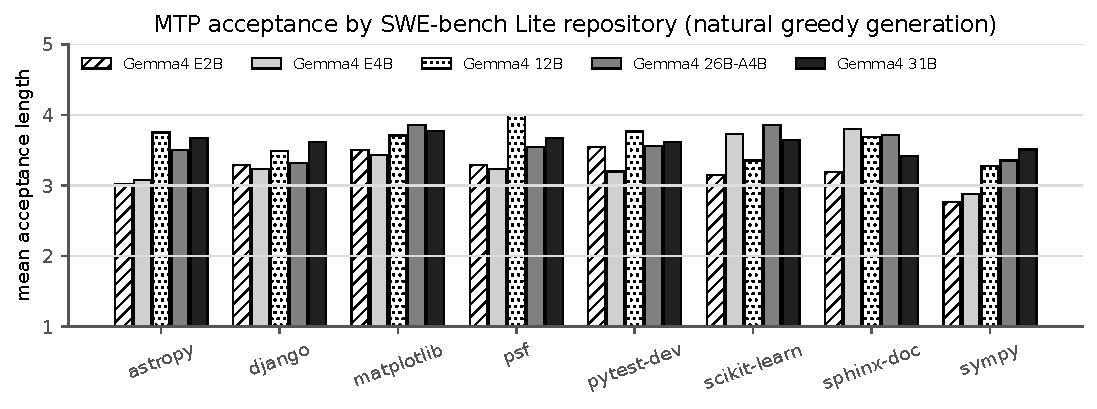
\includegraphics[width=\linewidth]{mtp_swe_genre.pdf}
\caption{SWE-bench Lite のリポジトリ別のmean acceptance length（$\gamma=4$，greedy 生成）．}
\label{fig:genre}
\end{figure}
\begin{figure}[htbp]\centering
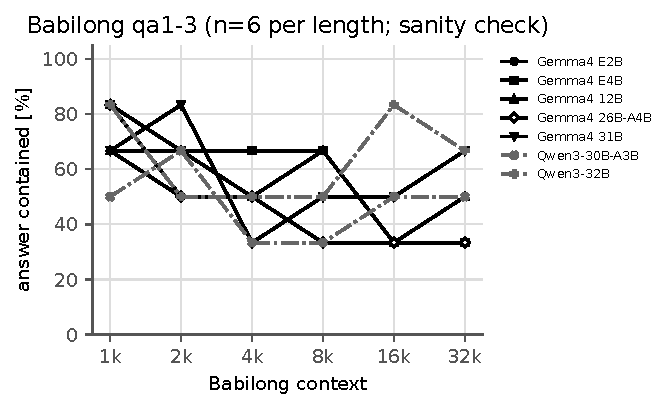
\includegraphics[width=0.6\linewidth]{babilong_accuracy.pdf}
\caption{Babilong qa1--qa3 の正答率（出力冒頭 80 文字に正解語を含む割合，各長さ 6 件）．
性能計測の健全性チェックであり，件数が少ないため精度の比較には使えない．}
\end{figure}
